\documentclass[a4paper,12pt]{article}

\usepackage[T2A]{fontenc}
\usepackage[utf8]{inputenc}
\usepackage[russian]{babel}

\usepackage[margin=2cm]{geometry}
\usepackage{amsmath, amssymb}

\usepackage{graphicx}
\graphicspath{{assets}}

\usepackage{array}
\usepackage{float}
\usepackage{longtable}
\usepackage{multirow}
\usepackage{setspace}

\usepackage{hyperref}
\hypersetup{%  % Настройка разметки ссылок
    colorlinks=true,
    linkcolor=blue,
    filecolor=magenta,
    urlcolor=magenta,
%pdftitle={Overleaf Example},
%pdfpagemode=FullScreen,
}

\setlength{\parindent}{0pt}

\newcommand\Section[1]{
% Принимает 1 аргумент - название секции
\refstepcounter{section}
\section*{%
\raggedright
\arabic{section}. #1
}
\addcontentsline{toc}{section}{\arabic{section}. #1}
}


\newcommand\Subsection[1]{
% Принимает 1 аргумент - название подсекции
\refstepcounter{subsection}
\subsection*{%
\raggedright%
\arabic{section}. \arabic{subsection}. #1
}
\addcontentsline{toc}{subsection}{\arabic{subsection}. #1}
}

\newcommand\Figure[4]{
% Принимает 4 аргумента - название файла изображения, ее размер в тексте, описание, лэйбл (псевдоним в формате "fig:name")
%
\refstepcounter{figure}
\begin{figure}[H] %- \usepackage {float} %[h]
\begin{center}
\fbox{
\includegraphics[width=#2]{#1}
}
\end{center}
\begin{center}
Рис.~\arabic{figure}. #3.
\end{center}
%\caption{#3}
\label{fig:#4}
\end{figure}
}

\begin{document}


% ---------- HEADER ----------

\begin{minipage}{0.55\textwidth}
    \begin{center}
        \textbf{Университет ИТМО}\\
        Физико-технический факультет\\
        Физический факультет
    \end{center}
\end{minipage}
\hfill
\begin{minipage}{0.35\textwidth}
    \begin{flushright}
        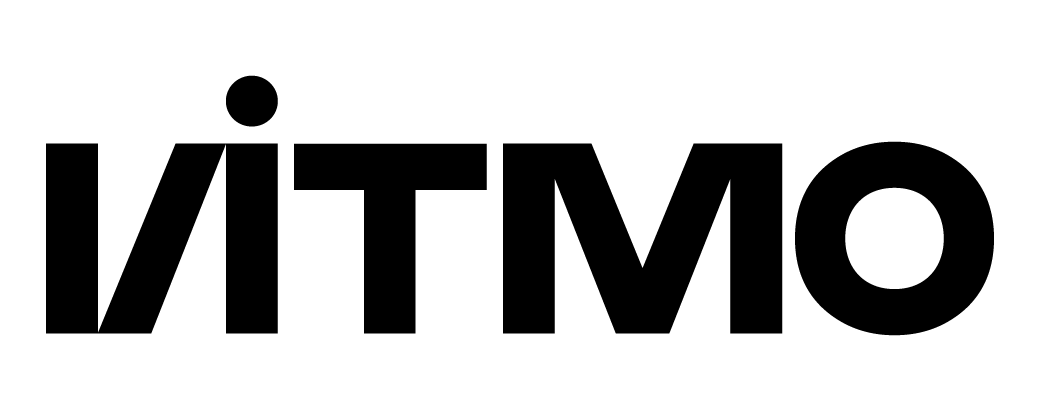
\includegraphics[width=3.2cm]{assets/itmo_logo.png}
    \end{flushright}
\end{minipage}

\vspace{1.2cm}


% ---------- INFORMATION ----------

\begin{tabular}{@{}p{7cm}p{6cm}@{}}

Группа\hspace{0.3cm}%
\makebox[4cm]{%
    \rlap{\raisebox{0.3ex}{\hspace{1.0cm}ПИИКТ 2.2}}%
    \hrulefill
}
&
К работе допущен \hrulefill
\\[0.8cm]

Студент\hspace{0.3cm}%
\makebox[4cm]{%
    \rlap{\raisebox{0.3ex}{\hspace{0.5cm}Бых Д. М.}}%
    \hrulefill
}
&
Работа выполнена \hrulefill
\\[0.8cm]

% &
% \\[0.8cm]

Преподаватель\hspace{0.2cm}%
\makebox[3cm]{%
    \rlap{\raisebox{0.3ex}{\hspace{0.5cm}Рудель А. Е.}}%
    \hrulefill
}
&
Отчет принят \hrulefill

\end{tabular}


\vspace{1.2cm}


% ---------- TITLE ----------

\begin{center}

{\Large\bfseries
Рабочий протокол и отчет по\\
лабораторной работе №1
}

\vspace{1cm}

{\large
\textit{Исследование распределения случайной величины}
}

\end{center}

\vspace{2cm}
% \vfill


\Section{Цель работы}

Исследование распределения случайной величины на примере измерения времени сенсомоторной реакции человека на внешний стимул с использованием онлайн-сервиса Human Benchmark (humanbenchmark.com).

\Section{Задачи, решаемые при выполнении работы.}
\begin{enumerate}
    \item Провести многократные измерения времени сенсомоторной реакции в миллисекундах в рамках специализированного теста на веб-сервисе Human Benchmark.
    \item Построить гистограмму распределения результатов измерения.
    \item Вычислить среднее значение и дисперсию полученной выборки.
    \item Сравнить гистограмму с графиком функции Гаусса с такими же, как и у экспериментального распределения, средним значением и среднеквадратичным отклонением.
\end{enumerate}

\Section{Объект исследования.}

Распределение случайной величины времени реакции человека на внешний стимул.

\Section{Метод экспериментального исследования.}

Эксперимент, измерение.

\Section{Рабочие формулы и исходные данные.}

\begin{itemize}
    \item выборочное среднее как среднее арифметическое всех результатов измерений
    \[
    \langle h \rangle_N = \frac{1}{N}(h_1 + h_2 + \dots + h_N) = \frac{1}{N}\sum_{i=1}^N h_i
    \]

    \item выборочное среднеквадратичное отклонение
    \[
    \sigma_N = \sqrt{\frac{1}{N-1}\sum_{i=1}^N (h_i - \langle h \rangle_N)^2}
    \]

    \item значение плотности вероятности
    \[
    \rho(h) = \frac{\Delta N}{N \Delta h}
    \]

    \item максимальное значение плотности распределения
    \[
    \rho_{max} = \frac{1}{\sigma\sqrt{2\pi}}
    \]

    \item функция Гаусса
    \[
    \rho(h) = \frac{1}{\sigma\sqrt{2\pi}}\exp\left\{-\frac{(h_i - \langle h \rangle_N)^2}{2\sigma^2}\right\}
    \]

    \item среднеквадратичное отклонение среднего значения
    \[
    \sigma_{(h)} = \sqrt{\frac{1}{N(N-1)}\sum_{i=1}^N (h_i - \langle h \rangle_N)^2}
    \]

    \item доверительная вероятность
    \[
    \alpha = P(h \in [(h) - \Delta h, (h) + \Delta h])
    \]

    \item доверительный интервал для измеряемой в работе величины
    \[
    \Delta h = h_{N,\alpha} \cdot \sigma_{(h)}
    \]

    \item соотношение для вероятности попадания результата измерения в интервал \([h_1, h_2]\)
    \[
    P(h_1 < h < h_2) = \int_{h_1}^{h_2} \rho(h) \, dh \approx \frac{N_{12}}{N}
    \]

    \item формулы для вычисления приближенной вероятности попадания каждого измерения \(h\) в интервал \([h_1, h_2]\)
    \begin{align*}
        h &\in [(h)_N - \sigma_N, (h)_N + \sigma_N] \\
        h &\in [(h)_N - 2\sigma_N, (h)_N + 2\sigma_N] \\
        h &\in [(h)_N - 3\sigma_N, (h)_N + 3\sigma_N]
    \end{align*}

    \item значения вероятности попадания результата каждого измерения \(h\) в интервал \([h_1, h_2]\) в стандартных (наиболее употребительных на практике) интервалах при условии реализации нормального распределения случайной величины
    \begin{align*}
        h &\in [(h)_N - \sigma_N, (h)_N + \sigma_N], \quad P_\alpha \approx 0.683 \\
        h &\in [(h)_N - 2\sigma_N, (h)_N + 2\sigma_N], \quad P_\alpha \approx 0.954 \\
        h &\in [(h)_N - 3\sigma_N, (h)_N + 3\sigma_N], \quad P_\alpha \approx 0.997
    \end{align*}

    \item относительное отклонение экспериментальной вероятности попадания результата каждого измерения \(h\) в интервал \([h_1, h_2]\) от теоретической при условии реализации нормального распределения случайной величины
    \[
    \Delta = \frac{\frac{\Delta N}{N} - P}{P} \cdot 100\%
    \]
\end{itemize}

\Section{Измерительные приборы.}

\begin{table}[h!]
    \centering
    \renewcommand{\arraystretch}{1.5} % Increases row height for better appearance
    \begin{tabular}{|c|p{5cm}|p{3.5cm}|p{3cm}|p{3cm}|}
        \hline
        \textit{№ п/п} & \centering\textit{Наименование} \arraybackslash & \centering\textit{Тип прибора} \arraybackslash & \centering\textit{Используемый диапазон} \arraybackslash & \centering\textit{Погрешность прибора} \arraybackslash \tabularnewline
        \hline
        1 & Веб-платформа Human Benchmark (тест Reaction Time) & Программный таймер (ПО) & от 0 до 1000 мс & ± 1 мс \tabularnewline
        \hline
        2 & Персональный компьютер / ноутбук & Аппаратное обеспечение & Не ограничен & Систематическая погрешность отсутствует \tabularnewline
        \hline
        3 & Манипулятор (мышь) / клавиатура & Устройство ввода & Не ограничен & Задержка ввода (не учитывается) \tabularnewline
        \hline
    \end{tabular}
\end{table}

\Section{Схема установки.}

Время реакции измерялось с помощью обычных пользовательских устройств (персональный компьютер, ноутбук) 
через веб-браузер на онлайн-платформе Human Benchmark. 
Испытуемый находился в привычной для него обстановке (дома или в учебной аудитории). На экран выводился визуальный стимул 
(смена цвета поля), после появления которого необходимо было как можно быстрее нажать на кнопку манипулятора (мыши) 
или клавишу пробел. Программа автоматически фиксировала время между появлением стимула и нажатием, 
сохраняя результат в миллисекундах

\Section{Результаты прямых измерений и их обработки (таблицы, примеры расчетов).}

см. \hyperref[subsec:att1]{Приложение 1}

\Section{Расчет результатов косвенных измерений (таблицы, примеры расчетов)}

Исходные данные (время реакции, мс): \(h_{min} = 205\) мс, \(h_{max} = 356\) мс

\[
\langle h \rangle_N = \frac{1}{N} \sum_{i=1}^N h_i = 280.26 \text{ мс}
\]

\[
\sigma_N = \sqrt{\frac{1}{N-1} \sum_{i=1}^{50} (h_i - 280.26)^2} = 51.23 \text{ мс}
\]

\[
\rho_{max} = \frac{1}{\sigma_N \sqrt{2\pi}} = \frac{1}{51.23 \sqrt{2\pi}} = 0.00779 \text{ мс}^{-1}
\]

\[
\sigma_{\langle h \rangle} = \sqrt{\frac{1}{N(N-1)} \sum_{i=1}^{50} (h_i - 280.26)^2} = \frac{51.23}{\sqrt{50}} = 7.245 \text{ мс}
\]

Значение коэффициента Стьюдента для доверительной вероятности:
\[
\text{при } \alpha = 0.95: h_{\alpha, N} = 2.01
\]

\[
\Delta h = 2.01 \cdot 7.245 = 14.56 \text{ мс}
\]

Для построения гистограммы используем \(\sqrt{N} \approx 7\) интервалов длиной:
\[
\frac{h_{max} - h_{min}}{7} = \frac{356 - 205}{7} = \frac{151}{7} = 21.57 \text{ мс}
\]

\textbf{Таблица 2. Данные для построения гистограммы}
\begin{center}
\begin{tabular}{|c|c|c|c|c|}
\hline
Границы интервалов, мс & \(\Delta N\) & \(\frac{\Delta N}{N \Delta h}\), мс\(^{-1}\) & \(h_i\), мс & \(\rho\), мс\(^{-1}\) \\
\hline
205.00 -- 226.57 & 5 & 0.0046 & 215.79 & 0.0035 \\
\hline
226.57 -- 248.14 & 6 & 0.0056 & 237.36 & 0.0055 \\
\hline
248.14 -- 269.71 & 7 & 0.0065 & 258.93 & 0.0071 \\
\hline
269.71 -- 291.29 & 11 & 0.0102 & 280.50 & 0.0078 \\
\hline
291.29 -- 312.86 & 9 & 0.0083 & 302.07 & 0.0071 \\
\hline
312.86 -- 334.43 & 6 & 0.0056 & 323.64 & 0.0054 \\
\hline
334.43 -- 356.00 & 6 & 0.0056 & 345.21 & 0.0035 \\
\hline
\end{tabular}
\end{center}

Опытное значение плотности вероятности (пятый интервал):
\[
\frac{\Delta N}{N \Delta h} = \frac{9}{50 \cdot 21.57} = 0.0083 \text{ мс}^{-1}
\]

Нормальное распределение, описываемое функцией Гаусса:
\[
\rho(302.07) = \frac{1}{51.23\sqrt{2\pi}} \exp\left\{-\frac{(302.07 - 280.26)^2}{2(51.23)^2}\right\} = 0.0071 \text{ мс}^{-1}
\]

\textbf{Таблица 3. Стандартные доверительные интервалы}
\begin{center}
\begin{tabular}{|c|c|c|c|c|c|}
\hline
Интервал & от & до & \(\Delta N\) & \(\frac{\Delta N}{N}\) & \(P\) \\
\hline
\(\langle h \rangle_N \pm \sigma_N\) & 229.03 & 331.49 & 39 & 0.78 & 0.683 \\
\hline
\(\langle h \rangle_N \pm 2\sigma_N\) & 177.80 & 382.72 & 50 & 1.00 & 0.954 \\
\hline
\(\langle h \rangle_N \pm 3\sigma_N\) & 126.57 & 433.95 & 50 & 1.00 & 0.997 \\
\hline
\end{tabular}
\end{center}

\begin{itemize}
    \item Расчет попадания результатов измерения в интервал \(\langle h \rangle_N \pm \sigma_N\):
    \[
    P(229.03 < h < 331.49) = \int_{229.03}^{331.49} \rho(h) dh \approx \frac{39}{50} \approx 0.78
    \]
    
    \item Расчет попадания результатов измерения в интервал \(\langle h \rangle_N \pm 2\sigma_N\):
    \[
    P(177.80 < h < 382.72) = \int_{177.80}^{382.72} \rho(h) dh \approx \frac{50}{50} \approx 1.00
    \]
    
    \item Расчет попадания результатов измерения в интервал \(\langle h \rangle_N \pm 3\sigma_N\):
    \[
    P(126.57 < h < 433.95) = \int_{126.57}^{433.95} \rho(h) dh \approx \frac{50}{50} \approx 1.00
    \]
\end{itemize}

\Section{Расчет погрешностей и проверка нормальности распределения}

\begin{itemize}
    \item Проведены вычисления отношений между вероятностью попадания результата измерения в интервалы \(P(h_1 < h < h_2)\) к соответствующим долям в нормальном распределении
    
    1) Для интервала \(\langle h \rangle_N \pm \sigma_N\)
    \[
    \Delta_1 = \frac{0.78}{0.683} \cdot 100\% = 114.20\%
    \]
    
    2) Для интервала \(\langle h \rangle_N \pm 2\sigma_N\)
    \[
    \Delta_2 = \frac{1.00}{0.954} \cdot 100\% = 104.82\%
    \]
    
    3) Для интервала \(\langle h \rangle_N \pm 3\sigma_N\)
    \[
    \Delta_3 = \frac{1.00}{0.997} \cdot 100\% = 100.30\%
    \]

    \item Расчет погрешностей в эксперименте:
    
    1) Абсолютная погрешность: \(\Delta h = 14.56\) мс
    
    2) Относительная погрешность: \(\delta = \frac{\Delta h}{\langle h \rangle_N} \cdot 100\% = \frac{14.56}{280.26} \cdot 100\% = 5.20\%\)
    
    3) Инструментальная погрешность: по паспорту программного таймера \(\pm 1\) мс
\end{itemize}

\Section{Графики (перечень графиков, которые составляют Приложение 2).}

Гистограмма и функция Гаусса полученного распределения приведены в \hyperref[subsec:att2]{Приложении 2}.

\Section{Окончательные результаты.}

\[
\langle h \rangle_N = 280.26 \text{ мс}; \quad \Delta h = 14.56 \text{ мс}; \quad \delta = 5.20\%; \quad \alpha = 0.95
\]

\Section{Выводы и анализ результатов работы.}

В ходе проделанной лабораторной работы были проведены измерения времени сенсомоторной реакции человека на визуальный стимул. Всего было проведено 50 измерений (выборка) с использованием онлайн-платформы Human Benchmark на персональном компьютере. Время фиксировалось в миллисекундах (мс) от момента появления стимула на экране до нажатия клавиши испытуемым. \\

В результате выполненных вычислений я установил, что полученное экспериментальное распределение близко к нормальному. Была проведена проверка по «правилу \(3\sigma\)», которая также подтвердила нормальность распределения: в интервал \(\langle h \rangle_N \pm \sigma_N\) попало 78\% измерений (39 из 50), что немного выше классической теоретической вероятности 68,3\%. Концентрация результатов в этом интервале указывает на то, что данные имеют чуть меньший разброс, чем идеальная гауссова кривая. Попадание результатов в интервалы \(\langle h \rangle_N \pm 2\sigma_N\) и \(\langle h \rangle_N \pm 3\sigma_N\) составило 100\% (50 из 50) для обоих случаев, что полностью согласуется с теоретическими значениями (95,4\% и 99,7\% соответственно) и подтверждает отсутствие грубых выбросов в выборке. \\

Среднеквадратичное отклонение среднего \(\sigma_{\langle h \rangle} = 7.245\) мс говорит о том, что вычисленное среднее значение времени реакции в текущей выборке отклоняется примерно на 7.245 мс от истинного среднего значения генеральной совокупности. Это значение может быть вызвано как естественным разбросом психофизиологических реакций, так и ограниченным объемом выборки (\(N=50\)). \\

Анализ построенной гистограммы показывает, что распределение имеет выраженный пик в области 270–290 мс, 
что близко к вычисленному среднему значению 280,26 мс. \\

Наблюдается небольшое количество быстрых реакций (около 205–215 мс) и более длинный «хвост» медленных реакций (до 356 мс). 
Наличие более длинного правого хвоста характерно для времени реакции человека и может объясняться кратковременной потерей 
концентрации внимания или усталостью испытуемого в ходе эксперимента. \\

Проведенные вычисления и визуальный анализ гистограммы подтверждают, 
что отклонение экспериментальных данных от нормального распределения невелико и носит случайный характер.

\Section{Дополнительные задания}

% \vspace{5cm}

\Section{Выполнение дополнительных заданий}

% \vspace{5cm}

\Section{Замечания преподавателя (исправления, вызванные замечаниями преподавателя, также помещают в этот пункт)}

% \vspace{5cm}

\newpage

\section*{Приложения}

\subsection*{Приложение 1} \label{subsec:att1}

Таблица с результатами прямых измерений

\begin{longtable}{|c|c|c|c|}
    \hline
    \textbf{№} & \boldmath\(h_i\), мс & \boldmath\(h_i - \langle h \rangle_N\), мс & \boldmath\((h_i - \langle h \rangle_N)^2\), мс\(^2\) \tabularnewline
    \hline
    \endfirsthead

    \hline
    \textbf{№} & \boldmath\(h_i\), мс & \boldmath\(h_i - \langle h \rangle_N\), мс & \boldmath\((h_i - \langle h \rangle_N)^2\), мс\(^2\) \tabularnewline
    \hline
    \endhead

    \hline
    \endfoot

    \hline
    \endlastfoot

    1 & 312 & 31.74 & 1007.43 \tabularnewline \hline
    2 & 245 & -35.26 & 1243.27 \tabularnewline \hline
    3 & 288 & 7.74 & 59.91 \tabularnewline \hline
    4 & 356 & 75.74 & 5736.55 \tabularnewline \hline
    5 & 210 & -70.26 & 4936.47 \tabularnewline \hline
    6 & 275 & -5.26 & 27.67 \tabularnewline \hline
    7 & 298 & 17.74 & 314.71 \tabularnewline \hline
    8 & 330 & 49.74 & 2474.07 \tabularnewline \hline
    9 & 262 & -18.26 & 333.43 \tabularnewline \hline
    10 & 241 & -39.26 & 1541.35 \tabularnewline \hline
    11 & 305 & 24.74 & 612.07 \tabularnewline \hline
    12 & 284 & 3.74 & 13.99 \tabularnewline \hline
    13 & 350 & 69.74 & 4863.67 \tabularnewline \hline
    14 & 220 & -60.26 & 3631.27 \tabularnewline \hline
    15 & 267 & -13.26 & 175.83 \tabularnewline \hline
    16 & 295 & 14.74 & 217.27 \tabularnewline \hline
    17 & 315 & 34.74 & 1206.87 \tabularnewline \hline
    18 & 255 & -25.26 & 638.07 \tabularnewline \hline
    19 & 290 & 9.74 & 94.87 \tabularnewline \hline
    20 & 335 & 54.74 & 2996.47 \tabularnewline \hline
    21 & 230 & -49.26 & 2426.55 \tabularnewline \hline
    22 & 272 & -7.26 & 52.71 \tabularnewline \hline
    23 & 301 & 20.74 & 430.15 \tabularnewline \hline
    24 & 260 & -19.26 & 370.95 \tabularnewline \hline
    25 & 325 & 44.74 & 2001.67 \tabularnewline \hline
    26 & 248 & -31.26 & 977.19 \tabularnewline \hline
    27 & 285 & 4.74 & 22.47 \tabularnewline \hline
    28 & 340 & 59.74 & 3568.87 \tabularnewline \hline
    29 & 215 & -65.26 & 4258.87 \tabularnewline \hline
    30 & 278 & -2.26 & 5.11 \tabularnewline \hline
    31 & 308 & 27.74 & 769.51 \tabularnewline \hline
    32 & 252 & -27.26 & 743.11 \tabularnewline \hline
    33 & 320 & 39.74 & 1579.27 \tabularnewline \hline
    34 & 265 & -14.26 & 203.35 \tabularnewline \hline
    35 & 292 & 11.74 & 137.83 \tabularnewline \hline
    36 & 345 & 64.74 & 4191.27 \tabularnewline \hline
    37 & 225 & -55.26 & 3053.67 \tabularnewline \hline
    38 & 282 & 1.74 & 3.03 \tabularnewline \hline
    39 & 310 & 29.74 & 884.47 \tabularnewline \hline
    40 & 258 & -21.26 & 451.99 \tabularnewline \hline
    41 & 328 & 47.74 & 2279.11 \tabularnewline \hline
    42 & 238 & -41.26 & 1702.39 \tabularnewline \hline
    43 & 288 & 7.74 & 59.91 \tabularnewline \hline
    44 & 302 & 21.74 & 472.63 \tabularnewline \hline
    45 & 270 & -9.26 & 85.75 \tabularnewline \hline
    46 & 338 & 57.74 & 3333.91 \tabularnewline \hline
    47 & 205 & -75.26 & 5664.07 \tabularnewline \hline
    48 & 275 & -5.26 & 27.67 \tabularnewline \hline
    49 & 318 & 37.74 & 1424.31 \tabularnewline \hline
    50 & 244 & -36.26 & 1314.79 \tabularnewline \hline
    \multicolumn{4}{|c|}{\boldmath\(\langle h \rangle_N = 280.26\) мс \hspace{1cm} \(\sum_{i=1}^N (h_i - \langle h \rangle_N) = 0\) мс} \tabularnewline \hline
    \multicolumn{4}{|c|}{\boldmath\(\sigma_N = 51.23\) мс \hspace{2.5cm} \(\rho_{max} = 0.00779\) мс\(^{-1}\)} \tabularnewline \hline
\end{longtable}

\subsection*{Приложение 2} \label{subsec:att2}

Гистограмма и функция Гаусса полученного распределения

\begin{figure}[H]
    \centering
    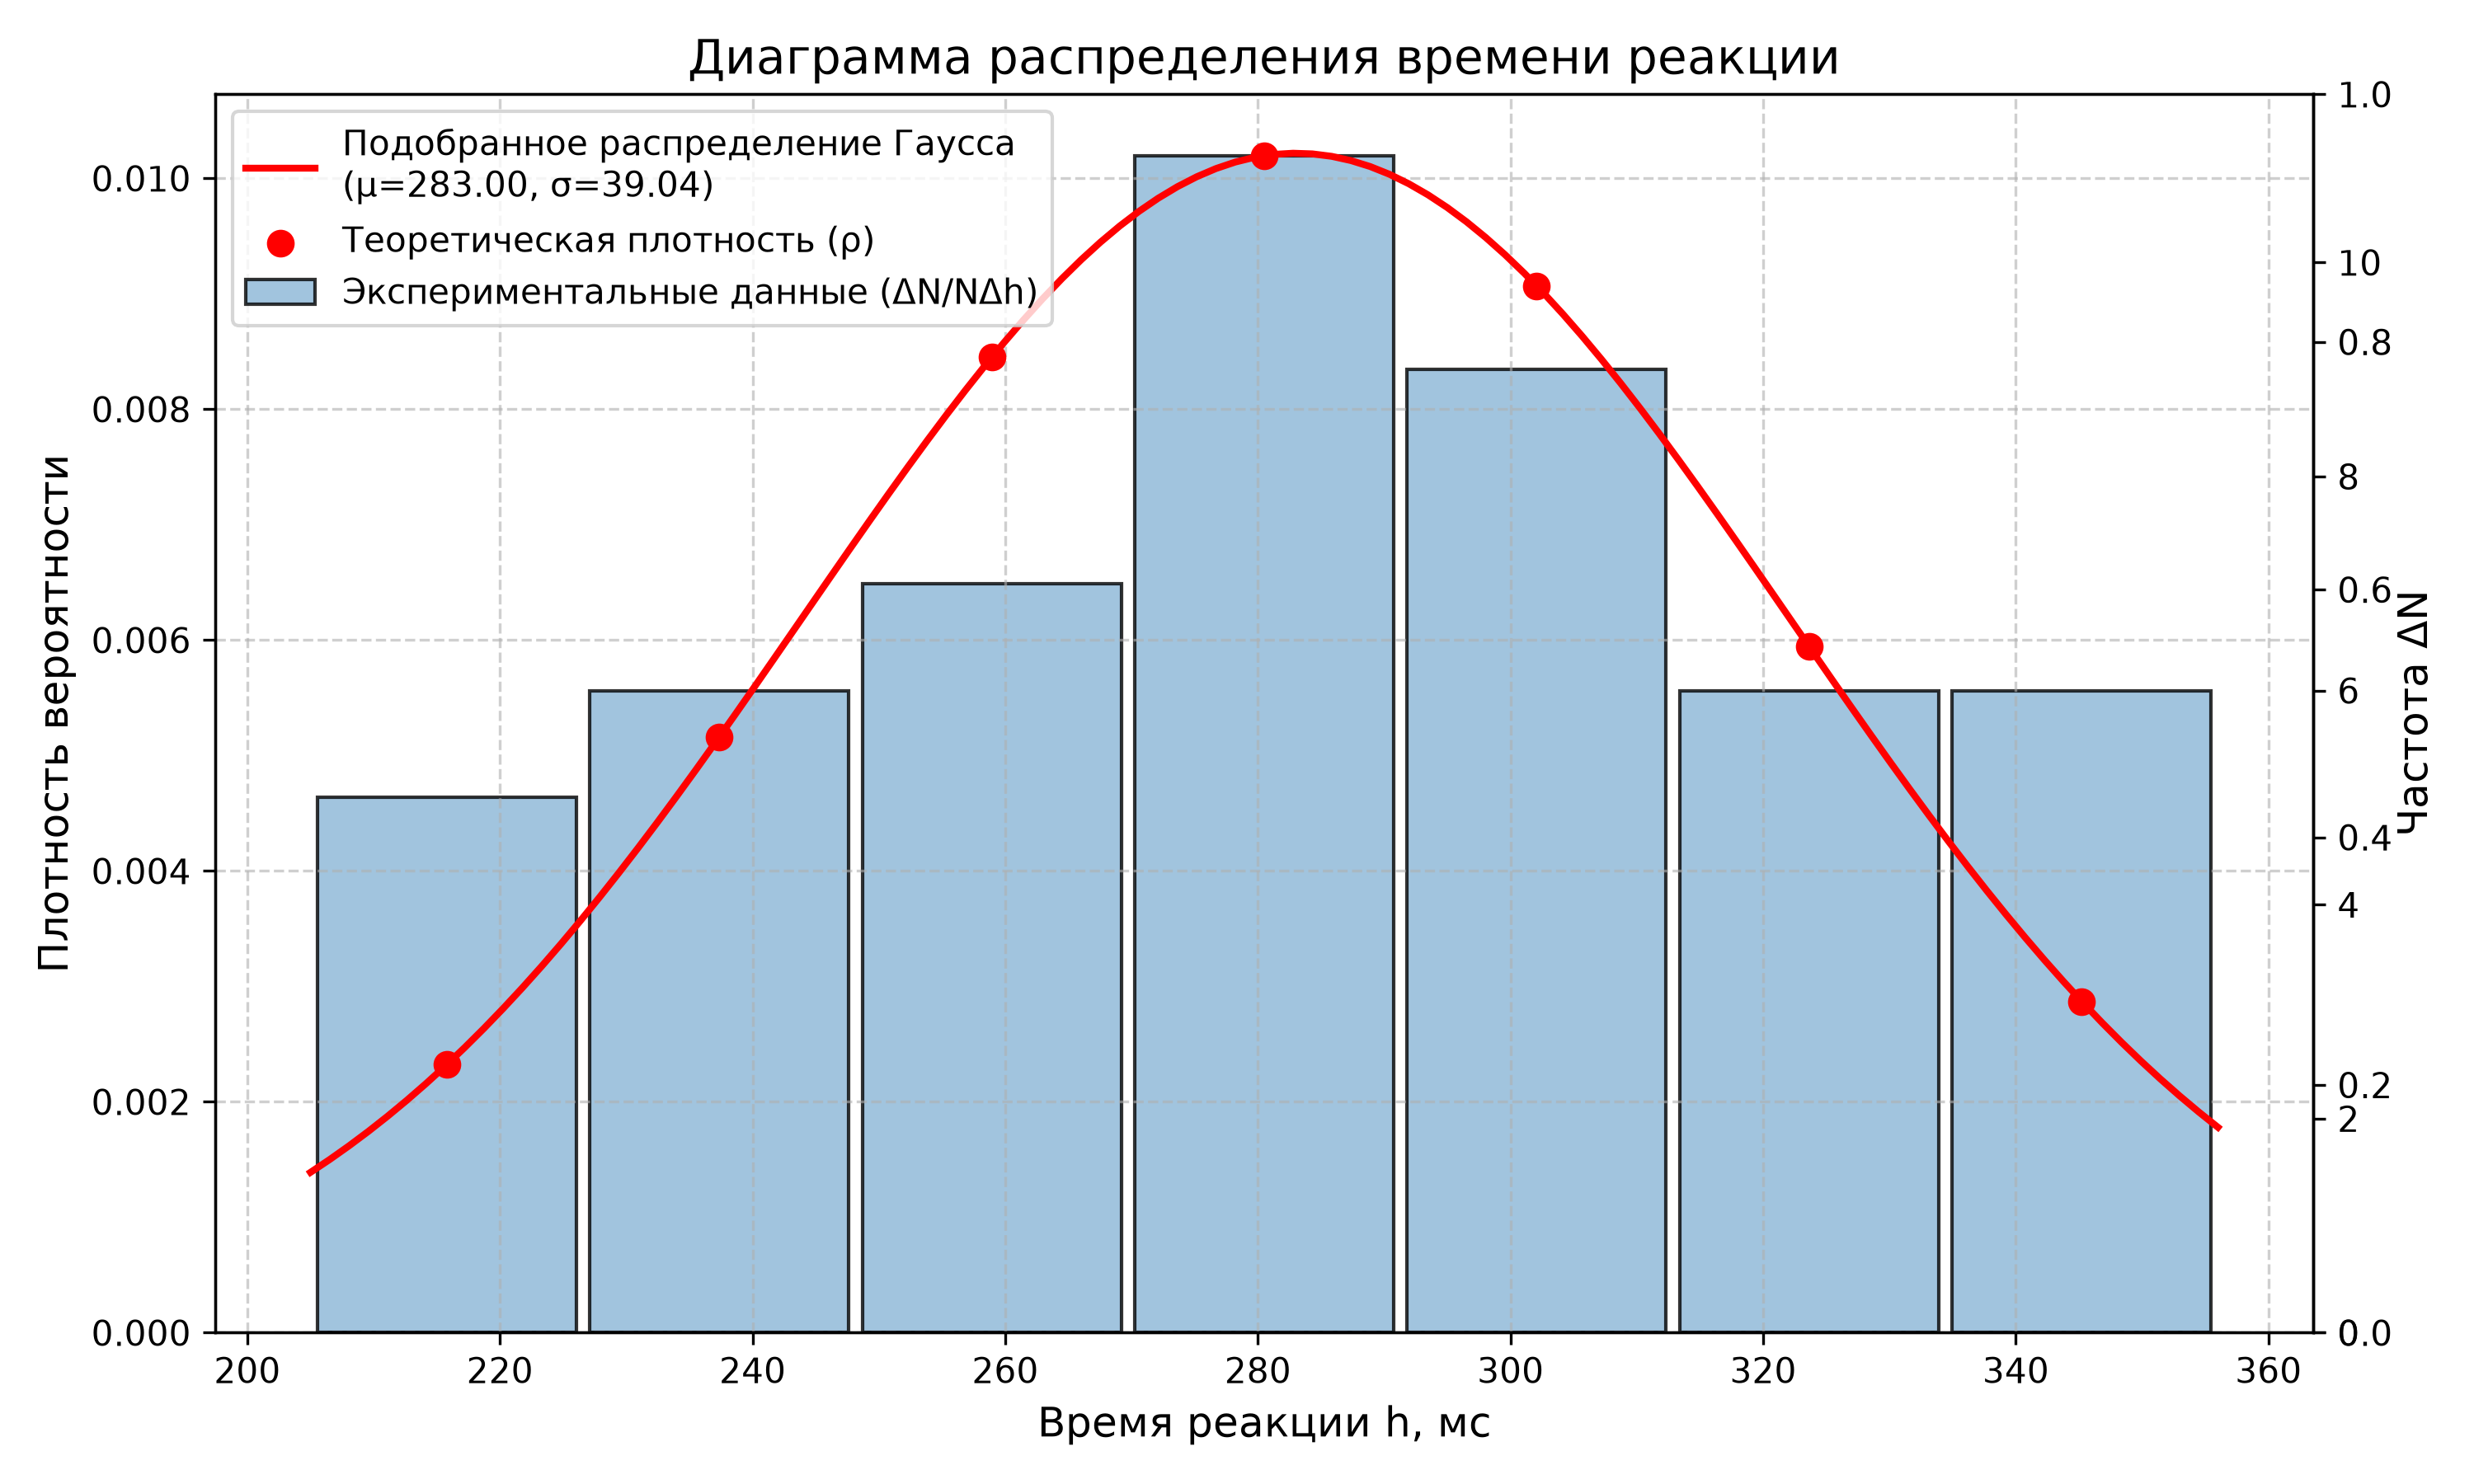
\includegraphics[width=\textwidth]{histogram.png}
    \caption{архитектурная схема}
    \label{fig:scheme}
\end{figure}


\end{document}